\section{Abstração e Representação da Lógica Computacional}

\subsection{O conceito de abstração em computação}

A abstração é considerada um dos conceitos fundamentais da Ciência da Computação, sendo utilizada para representar sistemas complexos por meio de modelos simplificados que destacam apenas os aspectos relevantes para determinado contexto. Segundo \citeonline{abelson1996}, a abstração permite que problemas computacionais sejam compreendidos e manipulados em diferentes níveis, reduzindo a necessidade de lidar diretamente com todos os detalhes de implementação, conforme a Figura \ref{fig:processo_abstracao}.

\begin{figure}[H]
    \centering
\caption{Processo de abstração aplicado à Ciência da Computação.}
    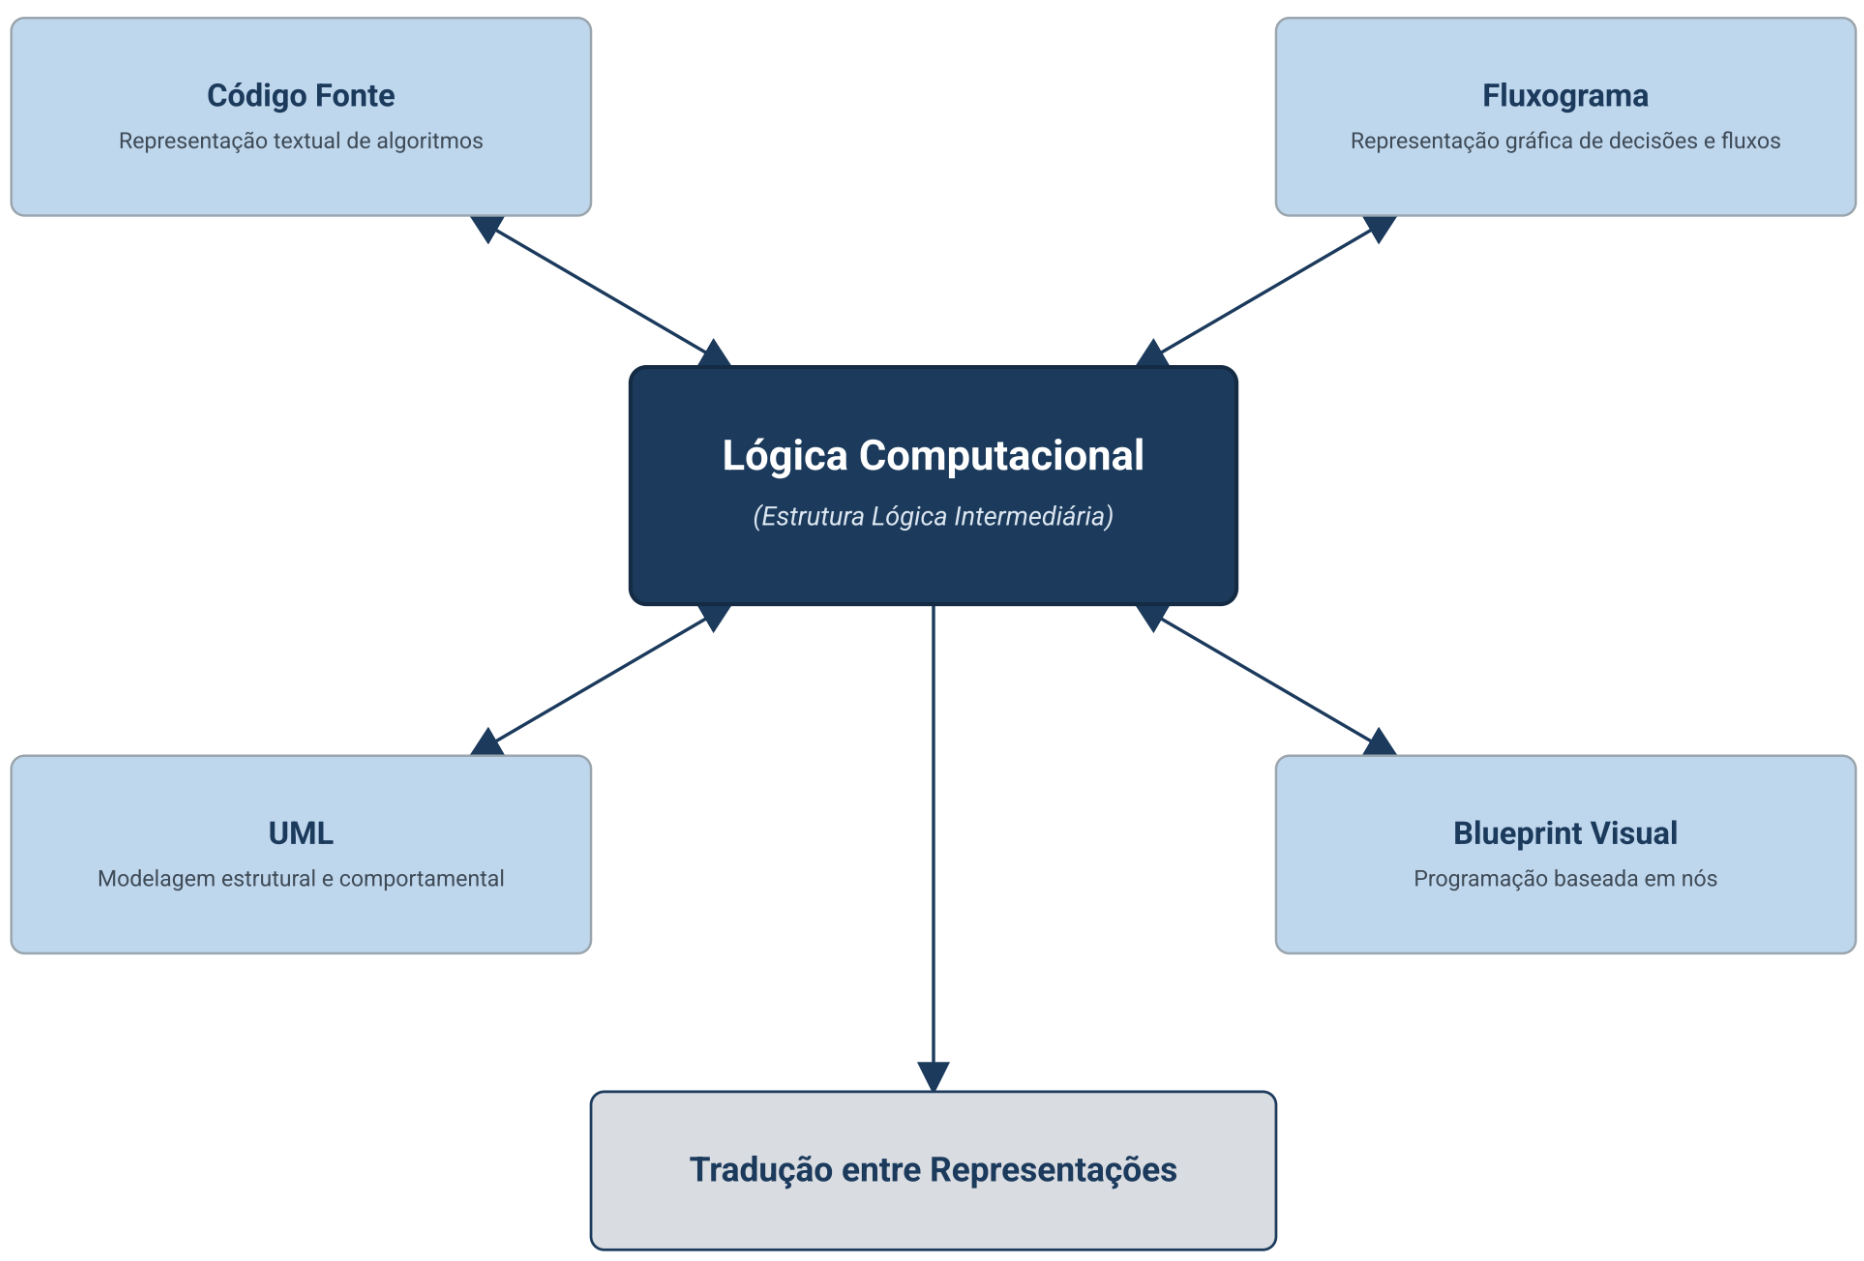
\includegraphics[width=\textwidth]{images/processo_abstracao.png}
\legend{Fonte: elaboração do autor com base em \citeonline{abelson1996}.}
    \label{fig:processo_abstracao}
\end{figure}


No desenvolvimento de software, a abstração está presente em diversas camadas, desde as linguagens de programação até as interfaces utilizadas pelos usuários finais. Cada camada oculta parte da complexidade da camada inferior, permitindo que desenvolvedores e usuários interajam com sistemas computacionais de maneira mais eficiente \cite{abelson1996}. Dessa forma, uma mesma lógica pode ser representada por diferentes mecanismos sem que seu significado fundamental seja alterado.

A compreensão desse conceito é especialmente relevante para esta pesquisa, uma vez que a hipótese investigada parte da possibilidade de que diferentes representações computacionais, como código textual e \textit{blueprints} visuais, possam expressar uma mesma estrutura lógica subjacente. Nesse contexto, a abstração torna-se um elemento central para compreender como a lógica computacional pode ser representada e interpretada em diferentes formatos.


\subsection{Lógica computacional independente da linguagem}

A lógica computacional pode ser compreendida como um conjunto de regras, decisões e processos que definem o comportamento de um sistema independentemente da linguagem utilizada para implementá-lo. Nesse contexto, as linguagens de programação atuam como mecanismos de representação dessa lógica, fornecendo estruturas sintáticas capazes de expressar algoritmos e comportamentos computacionais \cite{abelson1996}.

Segundo \citeonline{knuth1968}, os algoritmos constituem a base da computação, sendo independentes da tecnologia ou linguagem utilizada para sua implementação. Dessa forma, uma mesma solução lógica pode ser representada em diferentes linguagens de programação sem que seu objetivo fundamental seja alterado. O que muda é a forma de representação, enquanto a lógica subjacente permanece preservada.

Embora \citeonline{knuth1968} trate especialmente da independência entre algoritmos e linguagens textuais, esse mesmo princípio pode ser estendido às representações visuais. Uma decisão condicional, por exemplo, pode ser descrita por comandos em uma linguagem textual ou por elementos gráficos em fluxogramas e \textit{blueprints}, sem que a relação lógica entre a condição e seus possíveis fluxos de execução seja modificada. Dessa forma, a independência entre lógica e representação não se limita às linguagens de programação, estendendo-se também às formas visuais de representação computacional.

Essa independência entre lógica e representação, sustentada pelos conceitos de abstração de \citeonline{abelson1996} e pela noção de algoritmo de \citeonline{knuth1968}, constitui um dos fundamentos teóricos para investigar a viabilidade de traduções entre código textual e representações visuais. Compreender a lógica como uma estrutura separada de sua forma de representação é, portanto, condição necessária para analisar as relações existentes entre os diferentes modelos abordados nas seções seguintes.

\subsection{Representações da lógica computacional}

A lógica computacional pode ser expressa por diferentes modelos de representação, que variam conforme o contexto, o nível de abstração e os objetivos pretendidos. Ao longo da evolução da computação, essas formas foram desenvolvidas para atender a finalidades distintas, como facilitar a compreensão, documentar processos ou implementar sistemas executáveis.

Essas representações podem ser organizadas segundo diferentes critérios. Quanto à forma, distinguem-se as representações textuais (como o pseudocódigo e as linguagens de programação) das representações visuais (como os fluxogramas, os diagramas UML e os ambientes de programação baseados em nós). Quanto à finalidade, algumas representações possuem caráter essencialmente descritivo ou documental, voltado à compreensão e à comunicação de algoritmos, enquanto outras são executáveis, capazes de produzir diretamente o comportamento que descrevem. Apesar dessas diferenças, todas compartilham o objetivo comum de representar comportamentos, decisões e processos computacionais.

Essa diversidade de representações foi sistematizada por \citeonline{myers1990}, que propôs taxonomias para a programação visual e a visualização de programas, evidenciando que elementos gráficos podem representar relações e fluxos lógicos sem substituir a lógica computacional subjacente. Nessa perspectiva, a representação visual não se opõe ao código textual, mas oferece uma forma alternativa de expressar a mesma estrutura lógica.

A coexistência de múltiplas representações para uma mesma lógica sugere a existência de uma estrutura comum que as conecta. Compreender como cada modelo organiza e expressa algoritmos é, assim, um passo necessário para examinar as relações entre representações textuais e visuais, tema aprofundado na seção seguinte, dedicada à programação visual e aos ambientes baseados em fluxos.